\documentclass{article}

\usepackage[T1]{fontenc}
\usepackage[margin=1in]{geometry}
\usepackage{graphicx}
\usepackage{amsmath}
\usepackage{amssymb}
\usepackage{booktabs}
\usepackage{siunitx}
\usepackage{natbib}
\usepackage{subcaption}
\usepackage[hidelinks]{hyperref}

\newcommand{\keywords}[1]{\par\noindent\textbf{Keywords:} #1\par}

\title{Variance Retention as a Diagnostic Complement to Persistence-Relative
Skill in Multi-Horizon PM$_{10}$ Forecasting}
\author{Francisco Federico Garcia Crespi}
\date{July 2026}

\begin{document}

\maketitle

% ============================================================
\begin{abstract}
Persistence-relative RMSE skill is the standard yardstick for multi-horizon
point-forecast evaluation, but a skilled forecast under this criterion can
still be operationally uninformative if its predictions collapse toward a
near-constant value.
We evaluate multi-horizon PM$_{10}$ point forecasts under a rolling-origin
protocol with persistence as an explicit baseline, comparing LightGBM and
SARIMA across lead times $h \in \{1,6,24,48\}$ hours at an hourly-resolution
station in Madrid, Spain.
The leakage-free rerun does not reproduce the previously reported high skill:
LightGBM skill ranges from $-0.079$ to $0.073$, whereas SARIMA skill ranges
from $0.031$ to $0.132$.  Variance retention nevertheless changes the
interpretation of the positive SARIMA results: it falls from 79.8\% at
$h=1$ to 2.9\% and 0.4\% at $h=24$ and $48$, respectively.
We report horizon-wise variance retention alongside RMSE-based skill, and
introduce Skill$_{VP}$, a bounded diagnostic auxiliary that discounts nominal
skill by variance retention, to summarize this decoupling in a single
horizon-wise quantity.
Event-oriented evaluation under fold-recalibrated exceedance thresholds
confirms the horizon dependence: SARIMA recall falls from 0.785 at $h=1$ to
0.099 at $h=24$ and zero at $h=48$.  The results show why small positive
RMSE-relative skill should not be read as operational value without an
amplitude and event-detection diagnostic.
\end{abstract}

\keywords{PM$_{10}$ forecasting; multi-horizon forecasting; rolling-origin
evaluation; persistence baseline; forecast skill; variance retention;
dynamic fidelity}

% ============================================================
\section{Introduction}

Forecasts of particulate matter (PM$_{10}$) support operational activities
such as public health advisories, short-term compliance planning, and the
allocation of monitoring and mitigation resources \citep{donnelly2015}.
In such settings, model evaluation is often framed around useful lead times:
the range of horizons for which forecasts provide actionable information beyond
simple references.
Multi-horizon forecasting and horizon-wise verification are therefore standard
in air quality applications, and persistence remains a common baseline because
it is transparent and frequently competitive at short lead times
\citep{murphy1992}.

A practical complication is that squared-error criteria (MSE/RMSE) dominate
both model optimization and the reporting of multi-horizon performance.
Under limited predictability, point forecasts that shrink toward a central
tendency and dampen fluctuations can reduce squared error by avoiding large
misses, even if this also suppresses variability that may be operationally
relevant \citep{gneiting2011}.
This trade-off is well known in point forecasting under squared loss:
improvements in average error can coincide with reduced amplitude, and this
tension may become more salient as lead time increases and the conditional
distribution of outcomes broadens.

The gap addressed in this paper is empirical and protocol-specific.
In multi-horizon PM$_{10}$ forecasting evaluated with rolling-origin protocols,
positive persistence-relative RMSE skill can coexist with degraded dynamic
fidelity, reflected by a pronounced reduction in predicted variance relative to
observed variance at the same horizon.
In such cases, a horizon-wise skill curve may suggest that forecasts remain
useful at medium leads while the corresponding prediction sequences become
under-variable and less informative about episode evolution.
Rolling-origin evaluation is central to this diagnostic because it aggregates
performance over a sequence of forecast origins spanning changing conditions,
thereby exposing horizon-dependent behaviors that may be less visible under a
single blocked split \citep{tashman2000}.

This study provides a bounded empirical characterization of this decoupling
for LightGBM and SARIMA evaluated against a persistence baseline.
We report horizon-wise RMSE and persistence-relative skill together with
observed and predicted variances and variance retention, and we introduce
Skill$_{VP}$ as a simple diagnostic auxiliary metric to summarize how nominal
skill and variance retention jointly behave at each horizon.
The pattern in which persistence-relative RMSE skill remains positive while
predictive variance is substantially attenuated is sometimes described
informally in the forecasting community as ``ghost skill''; we use the term
here only as shorthand for that specific decoupling and do not adopt it as
formal terminology.

\paragraph{Contributions.}
The contribution is intentionally bounded and empirical:
\begin{itemize}
  \item We provide horizon-wise evidence, under rolling-origin evaluation with
    persistence as an explicit baseline, that persistence-relative RMSE skill
    can decouple from dynamic fidelity as measured by variance retention.
    LightGBM and SARIMA serve as contrasting cases: LightGBM does not
    consistently beat persistence, while SARIMA's modest positive skill at
    longer horizons coincides with severe variance attenuation and weak
    exceedance detection.
  \item We introduce Skill$_{VP}$ as a simple diagnostic auxiliary metric that
    adjusts nominal persistence-relative RMSE skill by variance retention for
    horizon-wise interpretation, and we report event-oriented complements
    (recall, precision, flag rate) under fold-recalibrated thresholds as a
    further check on operational usefulness.
\end{itemize}

% ============================================================
\section{Related Work and Positioning}

This manuscript is positioned as a restrained empirical-diagnostic study in
multi-horizon environmental forecasting.
It does not aim to advance general forecasting theory or introduce new universal
verification metrics.
Instead, it operationalizes several established verification ideas in a
deterministic PM$_{10}$ case study using a rolling-origin protocol,
persistence as an explicit baseline, horizon-by-horizon reading of skill, and
an explicit diagnosis of variance retention.

\subsection{Forecast skill and baseline-aware evaluation}

The horizon-wise perspective motivates treating the horizon as the primary unit
of interpretation in multi-step evaluation, rather than collapsing performance
into a single aggregate number \citep{bentaieb2012}.
In applied environmental forecasting, this framing is paired with explicit
reference forecasts that provide an operationally meaningful benchmark for
interpreting whether a model adds information beyond simple persistence-like
behavior \citep{murphy1992}.

The present paper adopts this baseline-aware, horizon-wise reading in a
deliberately narrow setting: deterministic point forecasts for PM$_{10}$
evaluated under a rolling-origin protocol with persistence as an explicit
baseline.
Rolling-origin aggregation preserves temporal causality and reduces the
optimistic bias that can arise when temporal dependence is insufficiently
respected, while also exposing horizon-dependent behavior across changing
conditions \citep{tashman2000}.

\subsection{Variance-fidelity diagnostics}

A well-known concern in deterministic point forecasting is that squared-error
optimization can encourage shrinkage toward conditional means, which may
suppress predictive variability as lead time increases \citep{gneiting2011}.
In environmental and hydrological verification, this issue connects to
antecedents that explicitly separate different components of performance,
including diagnostics that track variability ratios (e.g., the variability
component of KGE-style decompositions) and adjacent discussions of
oversmoothing and amplitude damping \citep{gupta2009,kling2012}.

The ingredients used here are classical: a baseline-relative skill quantity
and a variance ratio.
Letting $\mathrm{Skill}(h)$ denote persistence-relative RMSE skill at horizon
$h$ and letting $\sigma_{\hat{y}}^2(h)$ and $\sigma_y^2(h)$ denote the
horizon-wise predicted and observed variances over the rolling-origin
verification set, we define
\begin{equation}
  \mathrm{Skill}_{VP}(h) = \mathrm{Skill}(h)\,
  \frac{\sigma_{\hat{y}}^2(h)}{\sigma_y^2(h)},
\end{equation}
used here in a bounded form (see Section~\ref{sec:method_skillvp}).
Skill$_{VP}$ is positioned only as an auxiliary diagnostic complement that
down-weights nominal persistence-relative RMSE skill when variance retention
is low; its precise scope and boundaries are stated in
Section~\ref{sec:method_skillvp}.

\subsection{Contribution statement}

The strongest contribution of this paper is not conceptual novelty, but the
empirical combination of a PM$_{10}$ case study with rolling-origin evaluation,
persistence as an explicit operational baseline, horizon-by-horizon performance
reading, and an explicit variance-retention diagnosis.
In the reported results, LightGBM and SARIMA serve as contrasting cases:
LightGBM does not consistently improve on persistence, while SARIMA provides
the clearer case in which modest positive persistence-relative RMSE skill at
long horizons coexists with near-collapsed predictive variance.
This contrast motivates interpreting skill curves jointly with variance
retention when discussing horizon-wise usefulness, without claiming that such
decoupling must occur universally.

% ============================================================
\section{Methodology}

\subsection{Forecasting setting and multi-horizon notation}

Let $y_t$ denote the observed PM$_{10}$ concentration at time index $t$.
At each forecast origin $t$, a point forecasting model issues multi-horizon
predictions $\hat{y}_{t+h\mid t}$ for horizons $h \in \{1,\dots,H\}$.
Evaluation is performed separately for each horizon to avoid conflating
short- and long-lead behavior, since both error characteristics and the
operational interpretation of forecasts can change substantially with lead
time.

\subsection{Rolling-origin evaluation}

The empirical analysis was conducted on an hourly PM$_{10}$ series from the
Casa de Campo monitoring station in Madrid, Spain, covering the full calendar
year 2023 (2023-01-01 00:00 to 2023-12-31 23:00).  The regular hourly grid
contains 8,760 time stamps, of which 8,465 have measurements marked as valid
by the data provider; invalid or absent targets are excluded from verification.
The data were obtained from the Madrid Open Data portal operated by the
Ayuntamiento de Madrid.
Table~\ref{tab:data_protocol} summarises the study site, data coverage, and
evaluation protocol.

We adopt a rolling-origin (walk-forward) evaluation protocol to approximate
sequential operational use.
Models are refitted at the start of each expanding fold using only its training
window.  Within a test window, forecasts are issued sequentially using only
information available at origin $t$; the SARIMA state is updated without
parameter refitting when a new observation becomes available.
For each horizon $h$, verification aggregates over the set of valid origins
$\mathcal{T}_h$ with targets $y_{t+h}$ available, yielding horizon-wise sample
sizes $N_h = |\mathcal{T}_h|$.
This protocol avoids look-ahead and exposes the evaluation to changes in
conditions across origins \citep{tashman2000}.

\begin{table}[t]
\centering
\small
\caption{Summary of the study site, data coverage, and evaluation protocol.}
\label{tab:data_protocol}
\begin{tabular}{@{}ll@{}}
\toprule
Item & Value \\
\midrule
Study site / station       & Casa de Campo (Madrid, Spain) \\
Period                     & 2023-01-01 00:00 to 2023-12-31 23:00 \\
Temporal resolution        & 1 hour \\
Hourly grid / valid values & 8,760 / 8,465 \\
Data source                & Madrid Open Data, magnitude 10, station 024 \\
Forecast horizons ($h$)    & 1, 6, 24, 48 h \\
Rolling-origin folds       & 5 (expanding window, initial 50\%) \\
Holdout split              & 80/20 chronological \\
Models compared            & LightGBM; SARIMA \\
Baseline                   & Persistence \\
\bottomrule
\end{tabular}
\end{table}

\subsection{Reference forecast: persistence}

Persistence is used as an explicit baseline forecast.
For each origin $t$ and horizon $h$, the persistence prediction is
\begin{equation}
  \hat{y}^{(p)}_{t+h\mid t} = y_t.
\end{equation}
All skill statements in this paper are made relative to persistence and are
reported horizon-wise.

\subsection{Empirical models: LightGBM and SARIMA}

We report results for two empirical point-forecasting models.
The first is a gradient-boosted decision tree model (LightGBM), trained
independently for each fold and horizon $h$ using current and lagged values,
causal rolling-window statistics, and known calendar covariates \citep{ke2017}.
Unavailable inputs are forward-filled from the most recent valid observation;
backward filling is never used, and invalid targets are excluded.
LightGBM is included as a strong, widely used nonlinear predictor in applied
forecasting.

The second is SARIMA, a classical time-series model fitted on the raw PM$_{10}$
series at each rolling-origin fold using the fixed order
$(p,d,q)(P,D,Q)_s = (1,0,1)(1,0,0)_{24}$ recovered from the upstream experiment
configuration and recursive multi-step forecasting
\citep{boxjenkins2015}.
SARIMA is included not as a comprehensive statistical benchmark, but as a
comparator that can exhibit qualitatively different dynamic-fidelity behavior
under the same rolling-origin evaluation and persistence-relative skill framing.

\subsection{Horizon-wise RMSE and persistence-relative RMSE skill}

For model $m$ at horizon $h$, the rolling-origin RMSE is
\begin{equation}
  \mathrm{RMSE}_m(h) = \sqrt{\frac{1}{N_h}\sum_{t \in \mathcal{T}_h}
  \left(\hat{y}^{(m)}_{t+h\mid t}-y_{t+h}\right)^2}.
\end{equation}
Persistence-relative RMSE skill is defined as
\begin{equation}
  \mathrm{Skill}_{\mathrm{RMSE}}(h) = 1 -
  \frac{\mathrm{RMSE}_m(h)}{\mathrm{RMSE}_p(h)}.
\end{equation}
Positive values indicate lower RMSE than persistence at horizon $h$.

\subsection{Dynamic fidelity via variance retention}

To characterize amplitude preservation, we compute horizon-wise sample
variances over the same evaluation set $\mathcal{T}_h$:
\begin{equation}
  \mathrm{Var}_{\mathrm{obs}}(h)=
  \mathrm{Var}\!\left(\{y_{t+h}: t\in\mathcal{T}_h\}\right),
  \qquad
  \mathrm{Var}_{\mathrm{pred}}(h)=
  \mathrm{Var}\!\left(\{\hat{y}^{(m)}_{t+h\mid t}: t\in\mathcal{T}_h\}\right).
\end{equation}
Variance retention is reported as a percentage,
\begin{equation}
  \mathrm{VR}(h) = 100 \times
  \frac{\mathrm{Var}_{\mathrm{pred}}(h)}{\mathrm{Var}_{\mathrm{obs}}(h)}.
\end{equation}
Values substantially below 100\% indicate that predictions are under-variable
relative to observations at the same horizon.

\subsection{\texorpdfstring{Skill$_{VP}$}{SkillVP} as a diagnostic auxiliary metric}
\label{sec:method_skillvp}

RMSE-based skill and variance retention capture different aspects of forecast
behavior: the former summarizes average squared deviations, while the latter
summarizes amplitude preservation.
To characterize horizons where persistence-relative RMSE skill coexists with
low variance retention, we define Skill$_{VP}$ as a variance-preserving
diagnostic auxiliary:
\begin{equation}
  \mathrm{Skill}_{VP}(h) = \mathrm{Skill}_{\mathrm{RMSE}}(h)\times
  \min\!\left(1,\frac{\mathrm{Var}_{\mathrm{pred}}(h)}
  {\mathrm{Var}_{\mathrm{obs}}(h)}\right).
\end{equation}
The $\min(\cdot)$ bound prevents inflation when predictions are over-variable.
This construction is intentionally simple and is scoped narrowly: Skill$_{VP}$
is a horizon-wise diagnostic complement to RMSE-based skill, not a candidate
replacement for it, and it makes no claim about probabilistic calibration or
decision-theoretic optimality. Its sole purpose is to flag, at a glance,
horizons where nominal skill and amplitude preservation diverge.

% ============================================================
\section{Results}

\subsection{E1: Canonical horizon-wise results under rolling-origin evaluation}

Table~\ref{tab:canonical_results} and Figure~\ref{fig:skill_curve} report the
leakage-free rerun.  LightGBM does not consistently improve on persistence:
its skill is $-0.010$, $0.073$, $-0.034$, and $-0.079$ at
$h=1,6,24,48$.  SARIMA has modest positive skill at all four horizons
($0.031$--$0.132$), but its variance retention falls sharply with lead time,
from 79.8\% at $h=1$ to 35.7\% at $h=6$, 2.9\% at $h=24$, and 0.4\% at
$h=48$.  Thus the diagnostic issue is not an apparent equivalence between two
highly skilled models; it is the narrower observation that SARIMA's best
relative skill occurs where its predictive amplitude is least credible.

\begin{table}[t]
\centering
\small
\setlength{\tabcolsep}{5pt}
\caption{Canonical horizon-wise results under rolling-origin evaluation (E1).
  VR denotes variance retention (\%), and Skill$_{VP}$ is a diagnostic
  auxiliary adjustment of persistence-relative RMSE skill by variance
  retention.}
\label{tab:canonical_results}
\begin{tabular}{@{}rcccccccc@{}}
\toprule
& \multicolumn{4}{c}{LightGBM} & \multicolumn{4}{c}{SARIMA} \\
\cmidrule(lr){2-5}\cmidrule(lr){6-9}
$h$ & RMSE & Skill & VR (\%) & Skill$_{VP}$
    & RMSE & Skill & VR (\%) & Skill$_{VP}$ \\
\midrule
1 & 5.667 & $-0.010$ & 68.9 & $-0.007$ & 5.433 & 0.031 & 79.8 & 0.025 \\
6 & 9.147 & 0.073 & 55.1 & 0.040 & 9.050 & 0.083 & 35.7 & 0.029 \\
24 & 12.802 & $-0.034$ & 59.9 & $-0.021$ & 11.819 & 0.045 & 2.9 & 0.001 \\
48 & 15.228 & $-0.079$ & 86.6 & $-0.069$ & 12.241 & 0.132 & 0.4 & 0.000 \\
\bottomrule

\bottomrule
\end{tabular}
\end{table}

\begin{figure}[t]
\centering
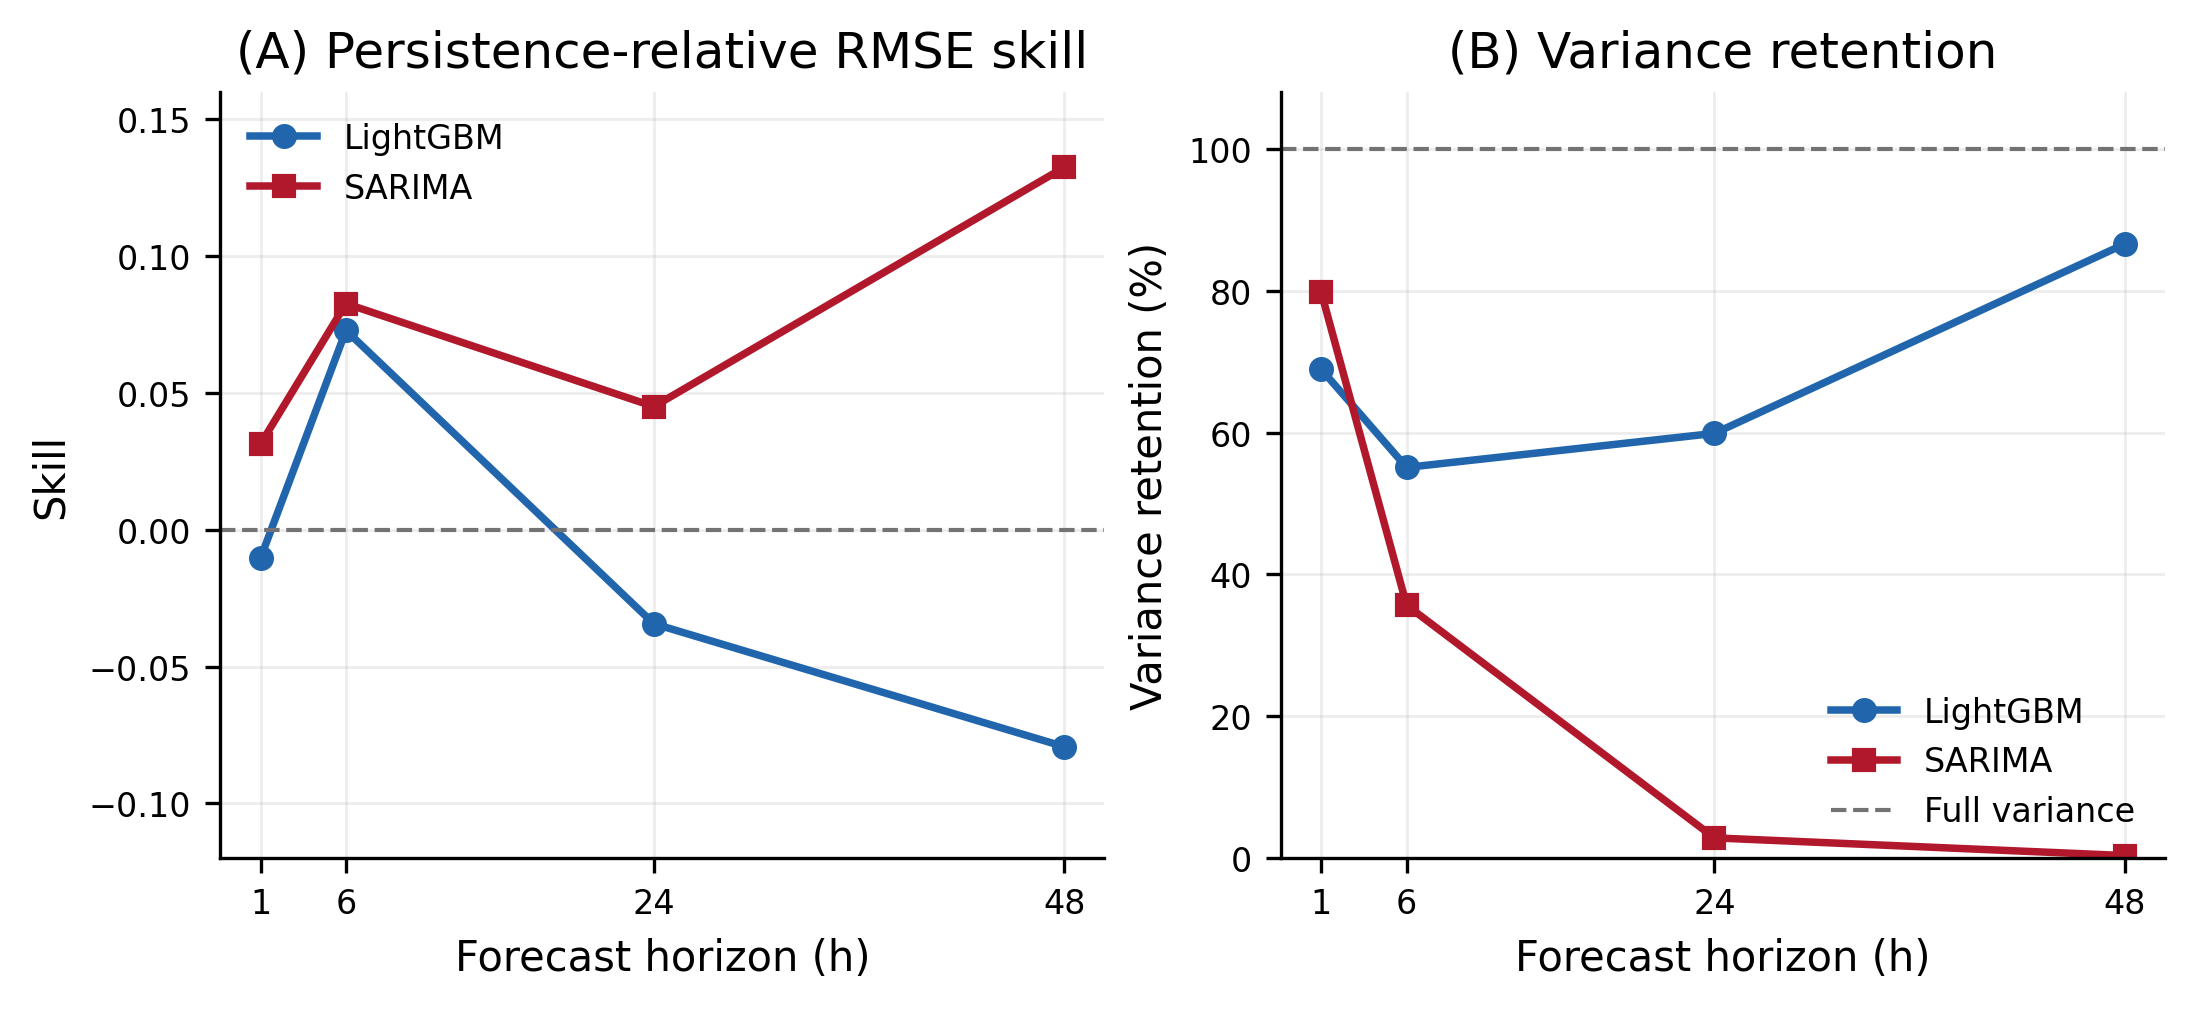
\includegraphics[width=0.95\linewidth]{outputs/figures/figure1_skill_variance.png}
\caption{Rolling-origin horizon-wise results for LightGBM and SARIMA.
  \textit{Left}: persistence-relative RMSE skill.
  \textit{Right}: variance retention (\%).
  SARIMA retains modest positive skill while its variance collapses at long
  horizons; LightGBM does not consistently beat persistence.}
\label{fig:skill_curve}
\end{figure}

\begin{figure}[t]
\centering
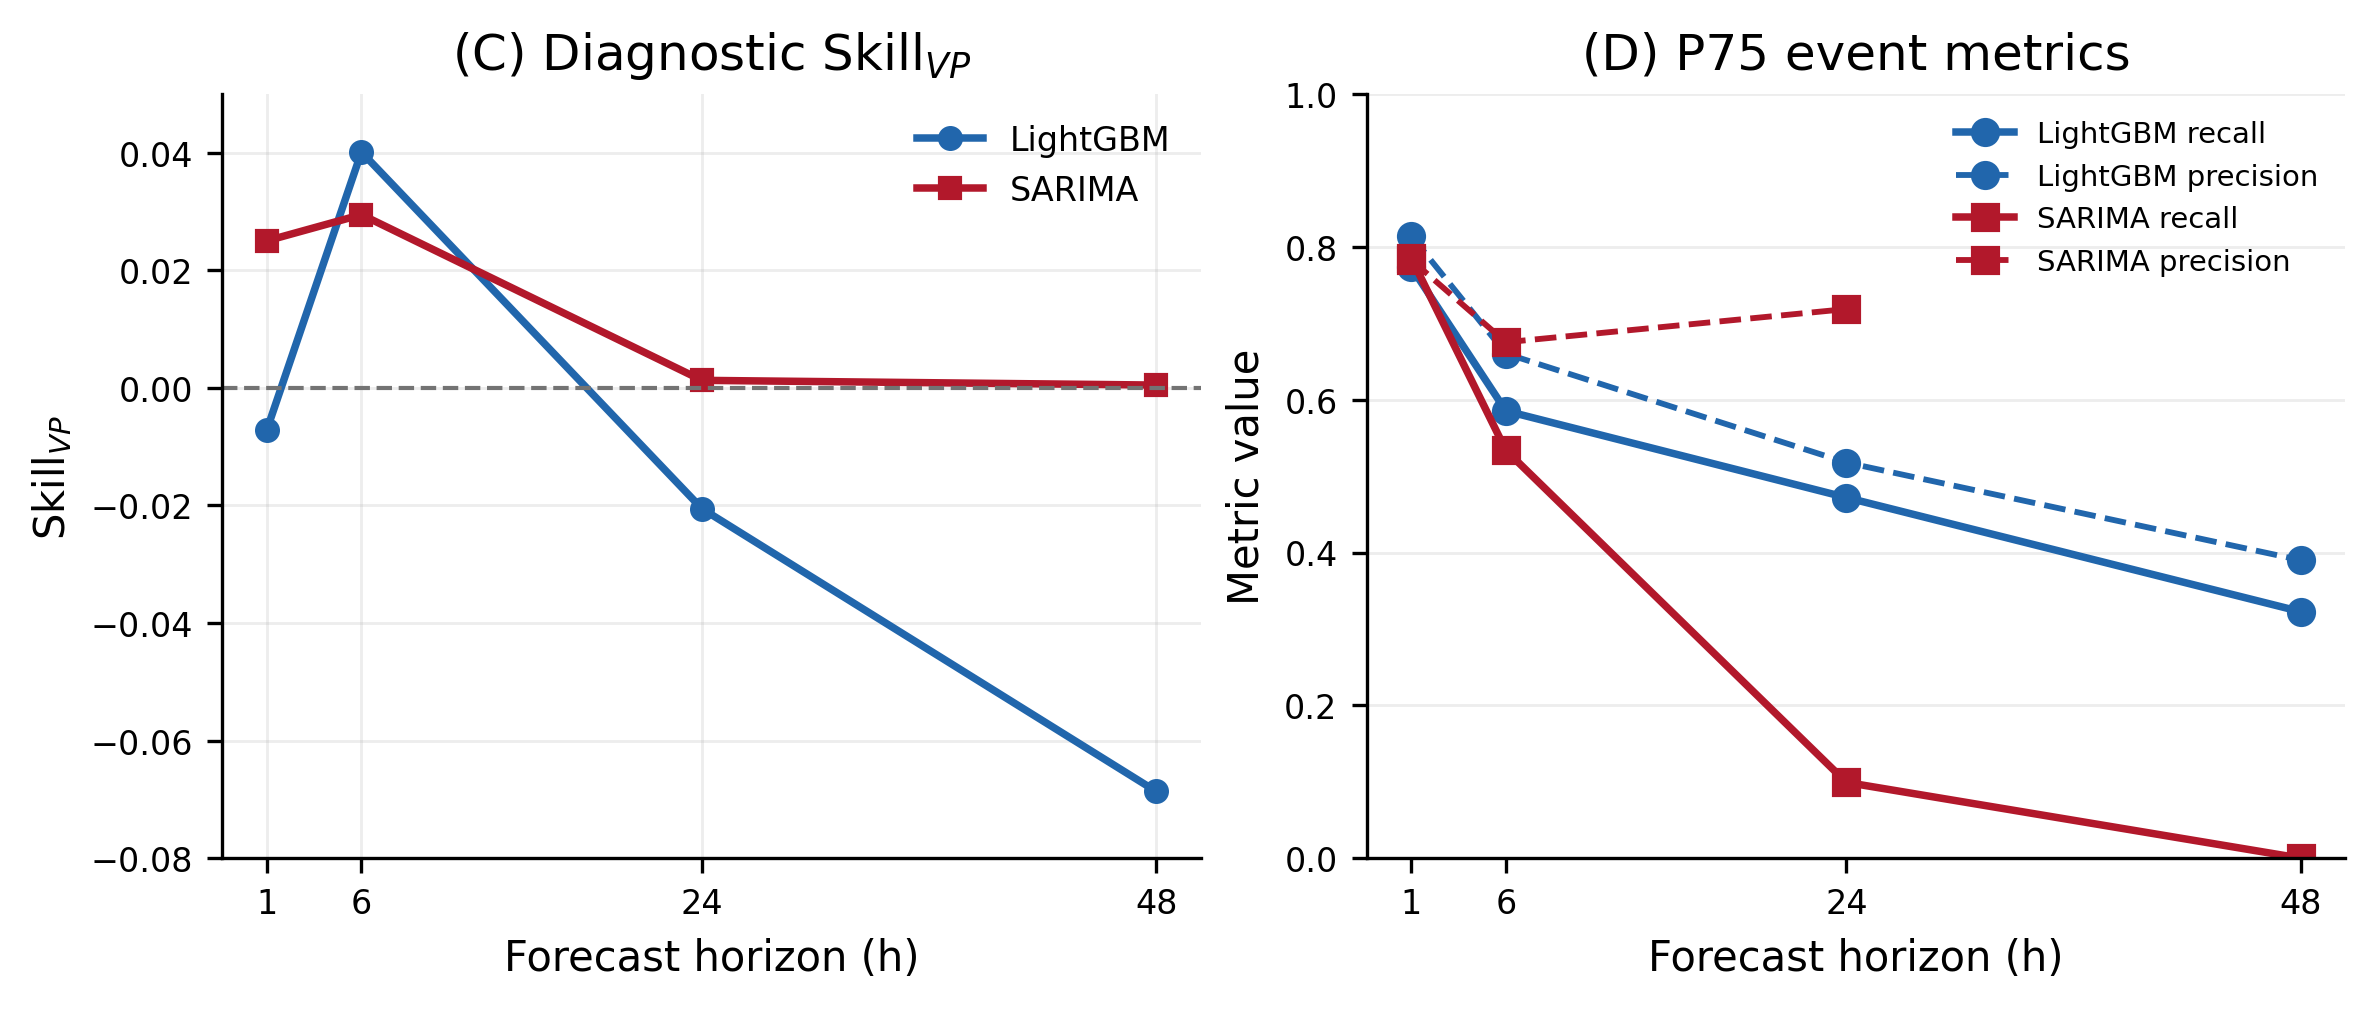
\includegraphics[width=0.95\linewidth]{outputs/figures/figure2_skillvp_events.png}
\caption{Diagnostic complements for horizon-wise interpretation.
  \textit{Left}: Skill$_{VP}$, which adjusts persistence-relative RMSE skill
  by variance retention.
  \textit{Right}: horizon-wise exceedance recall and precision at the P75
  threshold under fold-recalibrated evaluation.}
\label{fig:diagnostic_profiles}
\end{figure}

Skill$_{VP}$ makes this decoupling explicit per horizon by attenuating
persistence-relative RMSE skill when variance retention is low
(Figure~\ref{fig:diagnostic_profiles}, left).
For SARIMA, Skill$_{VP}$ falls from 0.025 and 0.029 at $h=1$ and $6$ to
0.001 and effectively zero at $h=24$ and $48$.  LightGBM's negative skill is
not rescued by variance retention: Skill$_{VP}$ remains non-positive except at
$h=6$ (0.040).

Importantly, the LightGBM results do not support a strong narrative of
long-horizon variance collapse within the currently evaluated range.
Variance retention is non-monotone for LightGBM and reaches 86.6\% at $h=48$.
The stronger diagnostic signal is model-dependent: SARIMA provides the clearer
extreme case, while LightGBM illustrates that amplitude preservation alone
cannot compensate for a lack of baseline-relative accuracy.

\subsection{E2: Protocol robustness (rolling-origin vs.\ blocked holdout)}

To assess whether the variance-retention contrast is specific to rolling-origin
aggregation, we report an analogous blocked-holdout evaluation.
The holdout results support the same qualitative long-horizon SARIMA pattern.
At $h=24$ and $48$, its variance retention is 3.35\% and 0.07\%, while skill
is $-0.029$ and 0.029.  LightGBM holdout skill is $-0.065$, 0.057,
$-0.062$, and 0.066, with variance retention of 79.5\%, 62.9\%, 68.2\%, and
32.6\%.  The sign and magnitude of skill are protocol-sensitive, but SARIMA's
long-horizon amplitude attenuation appears under both evaluations.

\subsection{E3: Event-oriented complement}

As a supportive operational complement, we evaluate exceedance detection at
the P75 threshold under fold-recalibrated thresholds (one threshold per
rolling-origin fold, fitted on that fold's training data).
LightGBM recall decreases from 0.773 at $h=1$ to 0.323 at $h=48$, with
precision decreasing from 0.815 to 0.390.  SARIMA recall decreases from 0.785
at $h=1$ to 0.099 at $h=24$ and zero at $h=48$; its flag rate likewise falls
from 0.300 to zero.  This long-horizon failure is consistent with its near-zero
variance retention.

These event-oriented results are treated as supportive diagnostics.
Recall alone can be trivially high under threshold saturation—when forecasts
remain above a permissive threshold at most time steps—and should therefore be
interpreted jointly with precision, flag rate, and variance retention.
Under fold-recalibrated thresholds, neither model sustains strong event
detection across all horizons, and SARIMA's long-horizon event detection is
especially limited by its inability to predict concentration peaks.

Overall, E1--E3 jointly support a bounded, model-dependent conclusion:
persistence-relative RMSE skill can remain positive while dynamic fidelity
differs markedly across models, and variance retention together with
Skill$_{VP}$ provides a practical diagnostic view of this divergence for
horizon-wise interpretation.

% ============================================================
\section{Discussion}

The evidence in this manuscript supports a diagnostic, horizon-wise
interpretation of multi-horizon PM$_{10}$ point forecasts under rolling-origin
evaluation with persistence as an explicit baseline.
LightGBM does not consistently improve on persistence, whereas SARIMA remains
modestly positively skilled in the rolling-origin evaluation.  The variance
diagnostics show that SARIMA's positive skill at $h=24$ and $48$ coincides with
near-collapsed predictive variance.  This result is consistent with the view
that even a positive error-based skill value can mask severe loss of amplitude,
and that horizon-wise interpretation changes when variance retention is
examined alongside RMSE-relative skill.

Skill$_{VP}$ is useful as a diagnostic auxiliary metric precisely because it
makes this divergence explicit and comparable across horizons without requiring
additional probabilistic infrastructure.
The LightGBM results do not support a monotone variance-collapse narrative,
although its negative skill at three horizons rules out claims of consistent
improvement over persistence.  SARIMA provides clearer evidence that modest
RMSE-relative skill can coexist with near-zero variance retention, and the
event-oriented evaluation confirms the operational consequence at long leads.

Event-oriented evaluation must be handled cautiously.
Recall alone may be trivially high under threshold saturation and does not by
itself demonstrate predictive discrimination or operational usefulness.
In this study, fold-recalibrated thresholds prevent artificial inflation of
event base rates, and recall is reported jointly with precision and flag rate.
Under these conditions, the event metrics support the same cautious conclusion
as the variance diagnostics: performance deteriorates with horizon for both
models, and SARIMA's positive long-horizon skill does not translate into peak
detection.

% ============================================================
\section{Limitations}

This study is intentionally limited in scope.
The empirical evidence is anchored in a single station, a single calendar
year, and five rolling-origin folds; external validity to other pollutants,
temporal resolutions, monitoring sites, or longer evaluation windows has not
been established.
The results are restricted to the evaluated horizons $h\in\{1,6,24,48\}$ and
to two model classes (LightGBM, SARIMA) with specific, fixed configurations;
neither model was tuned to compete for state-of-the-art accuracy, since the
goal is to characterize a decoupling pattern rather than to benchmark model
performance.
Skill$_{VP}$'s scope is stated in Section~\ref{sec:method_skillvp} and is not
repeated here; the metric has not been validated outside the present case
study, and its behavior under regimes with strong seasonality or structural
breaks remains untested.

% ============================================================
\section{Conclusion}

In this PM$_{10}$ case study evaluated under rolling-origin protocols with
persistence as an explicit baseline, the reproducible evidence is modest:
LightGBM does not consistently beat persistence, and SARIMA achieves only small
positive skill.  Nevertheless, SARIMA's variance retention falls to 2.9\% and
0.4\% at 24 and 48 hours, and its exceedance recall falls to 0.099 and zero.
Reporting variance retention alongside RMSE skill, and using Skill$_{VP}$ as a
diagnostic auxiliary metric, offers a practical way to make this divergence
explicit for horizon-wise interpretation under rolling-origin evaluation,
without implying a universal replacement for established verification practices.

% ============================================================
\section*{Data and Code Availability}

The analysis code, configuration files, and evaluation scripts used in this
study are available at
\url{https://github.com/fedeg-umh-es/varret-pm10-paper}.
Raw PM$_{10}$ data were obtained from the Madrid Open Data hourly air-quality
archive (\url{https://datos.madrid.es/dataset/201200-0-calidad-aire-horario})
and are available under CC BY 4.0.  The repository records the annual archive
URL and SHA-256 checksum and includes scripts that recover the station series
and reproduce predictions, metrics, event diagnostics, and figures.

\bibliographystyle{plainnat}
\begingroup
\small
\setlength{\bibsep}{2pt}
\bibliography{references}
\endgroup

\end{document}
